\documentclass[aspectratio=169,11pt]{beamer}
\usepackage{beamerucad}
\usepackage{listings}
\definecolor{ckw}{HTML}{2563AB}\definecolor{cst}{HTML}{2E8B57}\definecolor{ccm}{HTML}{8A8F98}
\lstdefinestyle{jv}{language=Java,basicstyle=\ttfamily\footnotesize,
 keywordstyle=\color{ckw}\bfseries,stringstyle=\color{cst},commentstyle=\color{ccm}\itshape,
 showstringspaces=false,columns=fullflexible,keepspaces=true,
 backgroundcolor=\color{ucadband!8},frame=leftline,framerule=2.5pt,rulecolor=\color{ucadband},
 xleftmargin=8pt,aboveskip=3pt,belowskip=1pt,basewidth=0.5em}
\lstset{style=jv}
\title{Architectures Logicielles — Séance 5}
\subtitle{L'asynchrone : RabbitMQ, ou l'art de ne plus mourir ensemble}
\author{Dr. El Hadji Bassirou TOURÉ}
\institute{Département de Mathématiques et Informatique\\ Faculté des Sciences et Techniques\\ Université Cheikh Anta Diop de Dakar}
\date{}
\setucadfoot{Architectures Logicielles --- Séance 5 \quad\textbullet\quad Dr. El Hadji Bassirou TOURÉ --- DMI/FST/UCAD}
\graphicspath{{figs/}}
\begin{document}

\begin{frame}[plain,noframenumbering]\titlepage\end{frame}

\begin{frame}{Objectifs de la séance}
\begin{ucaddef}[Contenu]
{\small Dernière séance : les événements du Lab 3 quittent la JVM et traversent le réseau via \textbf{RabbitMQ}. Les notifications consomment depuis une \textbf{queue durable} ; le module paiement déménage en \textbf{Python (pika)} — deuxième extraction du cours, cette fois \emph{asynchrone} : sans façade, sans timeout, sans 503. Et la démonstration miroir de la panne du Lab 4 : un consommateur éteint, ce sont des messages \textbf{qui attendent} — pas une panne.}
\end{ucaddef}
\begin{itemize}\small
  \item Comprendre le \textbf{broker} : exchange, queue durable, clé de routage, acquittement.
  \item Publier depuis Spring (\textbf{Spring AMQP}) et consommer depuis Python (\textbf{pika}).
  \item Éprouver la \textbf{résilience} : arrêt, attente, rattrapage — zéro message perdu.
  \item Savoir trancher, pour chaque intégration : \textbf{synchrone ou asynchrone ?}
\end{itemize}
\end{frame}

% #####################################################################
\section{Le bilan des blessures}

\begin{frame}{Trois douleurs, soigneusement conservées}
{\small Nous avons laissé trois blessures ouvertes — volontairement :}
\begin{itemize}\small
  \item \textbf{La panne synchrone (Lab 4)} : \texttt{livraison-service} éteint $\Rightarrow$ la confirmation meurt en 503. Compréhensible pour l'assignation (il \emph{faut} une réponse)... mais les SMS et le paiement, eux, n'exigeaient aucune réponse — pourquoi partager le sort de qui que ce soit ?
  \item \textbf{Le statut manuel} : la course atteint 100\,\%, le service \emph{sait} — et pourtant quelqu'un doit cliquer « Marquer livrée ».
  \item \textbf{L'état qui s'évapore} : le service redémarre, les courses s'oublient, la base dit le contraire. Deux vérités, aucune réconciliation.
\end{itemize}
\begin{ucadret}[Le diagnostic commun]
{\small Ces trois douleurs ont la même racine : nos services ne savent communiquer qu'\textbf{en direct et à l'instant}. Il leur manque un endroit où déposer un fait pour qu'il soit traité \emph{quand le destinataire pourra} — une \textbf{boîte aux lettres durable}.}
\end{ucadret}
\end{frame}

% #####################################################################
\section{Le broker}

\begin{frame}{L'idée simple : le téléphone et le message}
\begin{ucadex}[Deux façons de joindre quelqu'un]
{\small \textbf{L'appel téléphonique} : il faut que l'autre décroche, maintenant. S'il dort, téléphone éteint — échec, rappelez plus tard. \textbf{Le message WhatsApp} : vous l'envoyez et passez à autre chose. Son téléphone est éteint ? Le message \emph{attend}. À l'allumage, il reçoit \emph{tout}, dans l'ordre — rien ne s'est perdu.}
\end{ucadex}
{\small Dans notre lab, mot pour mot :}
\begin{itemize}\small
  \item l'appel téléphonique $=$ l'appel HTTP du Lab 4 : il faut que \texttt{livraison-service} « décroche » — sinon, 503 ;
  \item le message WhatsApp $=$ l'événement via RabbitMQ : le backend publie et \textbf{continue sa route} ;
  \item le téléphone éteint $=$ \texttt{paiement-service} arrêté : les messages \textbf{attendent} dans sa queue ;
  \item l'allumage $=$ le redémarrage : \textbf{rattrapage intégral}, dans l'ordre, zéro perte.
\end{itemize}
{\scriptsize (RabbitMQ est le serveur qui garde les messages — la « boîte » entre l'envoyeur et le destinataire.)}
\end{frame}

\begin{frame}{RabbitMQ : la boîte aux lettres durable}
\centering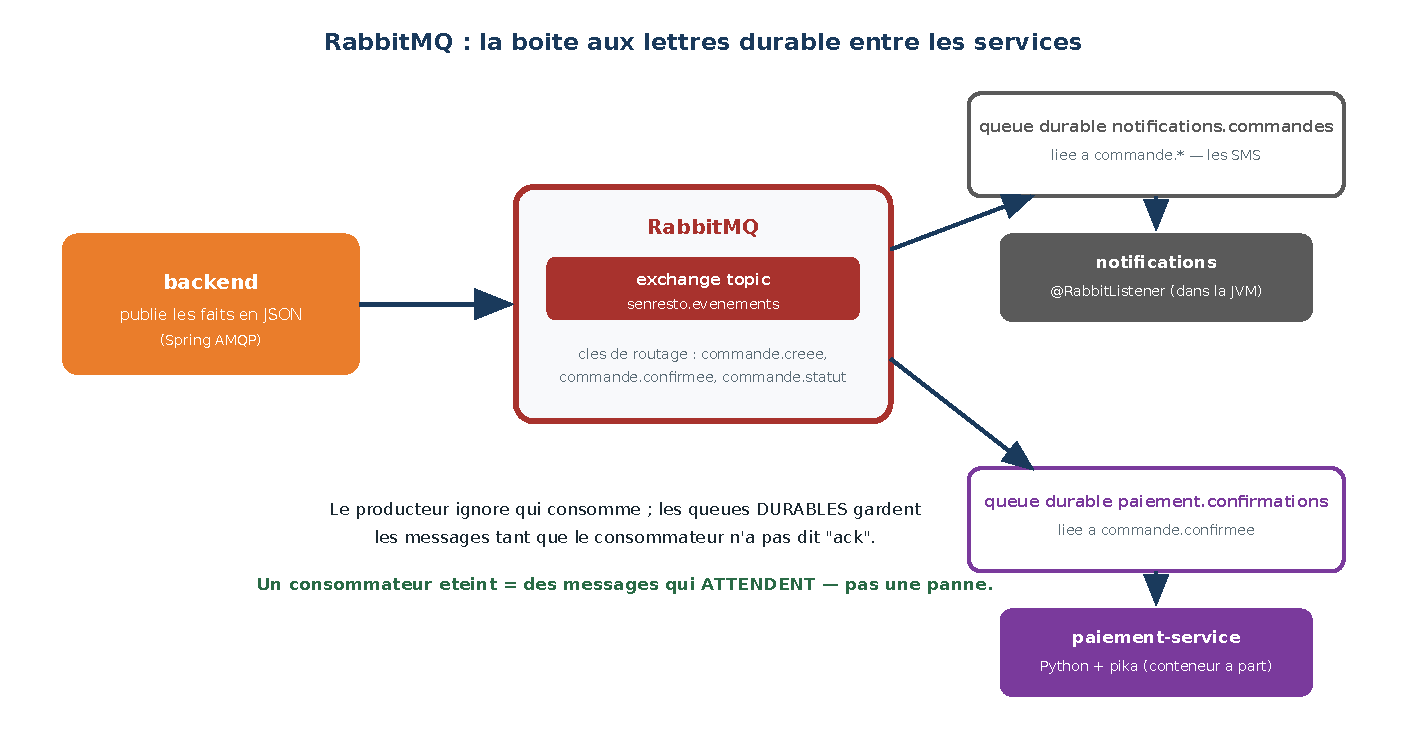
\includegraphics[width=0.80\linewidth]{figN_broker}
\end{frame}

\begin{frame}{Le trajet d'un message, pas à pas}
{\small Suivons \texttt{CommandeConfirmee} de bout en bout :}
\begin{enumerate}\small
  \item Le backend le dépose au \textbf{guichet de tri} (l'\emph{exchange} \texttt{senresto.evenements}) avec une \textbf{étiquette} (la \emph{clé de routage}) : \texttt{commande.confirmee}.
  \item Le guichet regarde qui s'est \textbf{abonné} (les \emph{bindings}) : la boîte des notifications a demandé « tout \texttt{commande.*} » ; celle du paiement, seulement \texttt{commande.confirmee}.
  \item Le message est \textbf{copié} dans chaque boîte concernée (les \emph{queues}) — une copie par abonné, chacun la sienne.
  \item Chaque consommateur relève \textbf{sa} boîte, à son rythme — réveillé ou pas au moment de l'envoi, peu importe.
\end{enumerate}
\begin{ucadret}[À retenir]
{\small Le backend ne connaît que le guichet et l'étiquette. Il ignore \textbf{qui} est abonné, \textbf{combien} ils sont, et \textbf{s'ils sont réveillés}. C'est le découplage du Lab 3 — étendu au réseau et au temps.}
\end{ucadret}
\end{frame}

\begin{frame}{Qui reçoit quoi ? Le routage en pratique}
{\small Nos trois étiquettes face à nos deux boîtes :}
\vskip2pt
{\small\begin{tabular}{p{0.30\linewidth}cc}
\toprule
\textbf{Clé du message} & \textbf{notifications} & \textbf{paiement}\\
 & (abonnée à \texttt{commande.*}) & (abonnée à \texttt{commande.confirmee})\\
\midrule
\texttt{commande.creee} & reçoit & ---\\
\texttt{commande.confirmee} & reçoit & reçoit\\
\texttt{commande.statut} & reçoit & ---\\
\bottomrule
\end{tabular}}
\vskip4pt
\begin{itemize}\small
  \item Le \texttt{*} de l'abonnement remplace \textbf{un mot} : \texttt{commande.*} attrape les trois clés.
  \item Demain, un module statistiques s'abonne à \texttt{commande.\#} : \textbf{zéro modification} chez le backend — comme le module paiement du Lab 3, version réseau.
\end{itemize}
\end{frame}

\begin{frame}{Le vocabulaire qui suffit}
{\small\begin{tabular}{p{0.22\linewidth}p{0.68\linewidth}}
\toprule
\textbf{Exchange} & le guichet de tri : reçoit chaque message et le route\\
\textbf{Clé de routage} & l'étiquette du message (\texttt{commande.confirmee})\\
\textbf{Queue durable} & la boîte d'un consommateur ; survit aux redémarrages\\
\textbf{Binding} & l'abonnement d'une queue (\texttt{commande.*} = tout)\\
\textbf{Ack} & l'accusé du consommateur ; sans lui, le message reste\\
\bottomrule
\end{tabular}}
\vskip4pt
\begin{ucadret}[À retenir]
{\small Cinq mots, et vous savez lire l'UI de gestion de RabbitMQ — votre poste d'observation de tout le lab. La garantie qu'ils construisent ensemble arrive à la slide suivante.}
\end{ucadret}
\end{frame}

\begin{frame}{L'ack : pourquoi APRÈS le traitement ?}
{\small L'\emph{ack} est l'accusé de réception du consommateur. Tout tient dans \textbf{le moment} où on l'envoie. Deux scénarios de crash :}
\begin{itemize}\small
  \item \textbf{Ack \emph{avant} de traiter} : le consommateur acquitte, la queue efface le message... et le consommateur crashe avant d'avoir traité. Le message est \textbf{perdu pour toujours} — un encaissement envolé.
  \item \textbf{Ack \emph{après} avoir traité} (notre règle) : le consommateur crashe en plein traitement ? Pas d'ack reçu — la queue \textbf{redonne le message} au redémarrage. Rien ne se perd... mais le message peut être \textbf{livré deux fois}.
\end{itemize}
\begin{ucaddef}[La garantie \emph{at-least-once}]
{\small Queue durable + message persistant + ack après traitement = chaque message est livré \textbf{au moins une fois}, à travers pannes et redémarrages. « Au moins » — donc \emph{parfois deux fois} : c'est un choix, pas un défaut. L'alternative (au plus une fois) accepte de \textbf{perdre} des messages — inacceptable pour un paiement.}
\end{ucaddef}
\end{frame}

% #####################################################################
\section{Publier et consommer}

\begin{frame}[fragile]{Publier : le pont vers le broker}
{\small Nos modules publient déjà des faits (Lab 3). Un \textbf{pont} suffit — il écoute les événements internes et les réexpédie en JSON :}
\begin{lstlisting}
@Component
class PontAmqp {
    private final RabbitTemplate rabbit;
    // ...
    @EventListener
    void quandCommandeConfirmee(CommandeConfirmee evt) {
        rabbit.convertAndSend("senresto.evenements",   // exchange
                "commande.confirmee",                  // cle de routage
                evt);                                  // serialise en JSON
    }
}
\end{lstlisting}
\begin{itemize}\small
  \item \texttt{CommandeMetier} n'a \textbf{pas bougé} d'une ligne : il publie ses faits comme au Lab 3, sans savoir qu'un pont les fait désormais voyager. Les frontières du modulith paient une dernière fois.
\end{itemize}
\end{frame}

\begin{frame}[fragile]{Consommer côté Java : notifications}
{\small Côté monolithe, notifications troque son \texttt{@EventListener} contre une queue durable — le Strangler, encore : l'ancien chemin reste sous \texttt{@Profile("!amqp")}, le nouveau vit sous \texttt{@Profile("amqp")} :}
\begin{lstlisting}
@RabbitListener(queues = "notifications.commandes")
void surEvenement(Map<String, Object> evt,
        @Header("amqp_receivedRoutingKey") String cle) {
    // memes textes de SMS qu'avant, aiguilles par la cle
}
\end{lstlisting}
\begin{itemize}\small
  \item La queue est déclarée \textbf{durable} : elle survit aux redémarrages — du broker comme du consommateur.
  \item Ce qui change pour l'utilisateur : \textbf{rien}. Mêmes SMS, même ordre. Ce qui change pour l'architecte : les SMS ne peuvent \textbf{plus se perdre}.
\end{itemize}
\end{frame}

\begin{frame}[fragile]{Consommer côté Python : le paiement déménage}
{\small Le paiement quitte le monolithe pour son propre conteneur — \textbf{pika}, le dialecte AMQP de Python :}
\begin{lstlisting}
def sur_message(canal, methode, proprietes, corps):
    evt = json.loads(corps)
    print(f"[PAIEMENT] Encaissement mobile money simule : "
          f"{evt['montantTotal']} FCFA pour {evt['numero']}")
    canal.basic_ack(methode.delivery_tag)   # l'ack APRES le traitement

canal.basic_consume(queue="paiement.confirmations", on_message_callback=sur_message)
\end{lstlisting}
\begin{ucadret}[La deuxième extraction — comparez au Lab 4 !]
{\small Extraire \texttt{paiement} n'a demandé \textbf{ni façade, ni timeout, ni 503} : personne n'attend sa réponse. L'extraction asynchrone est \emph{radicalement} moins chère — quand la nature de l'échange le permet.}
\end{ucadret}
\end{frame}

% #####################################################################
\section{La resilience}

\begin{frame}{La démonstration miroir}
\centering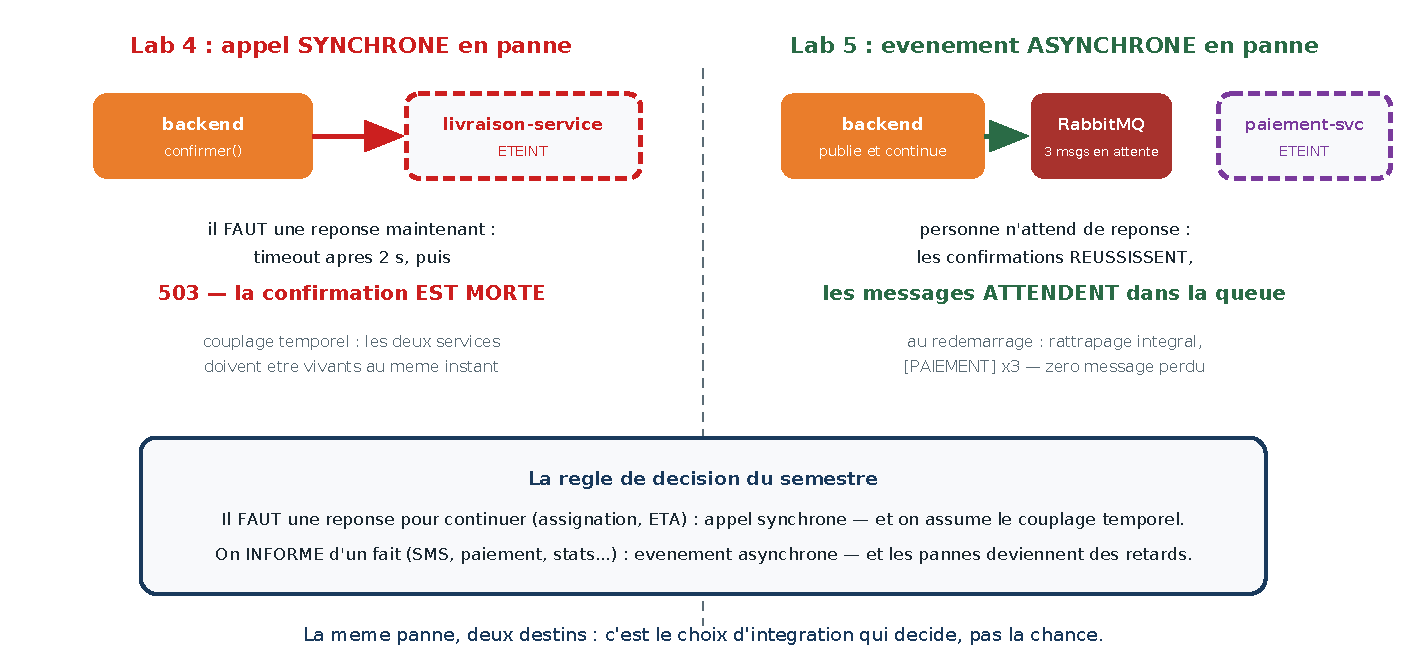
\includegraphics[width=0.86\linewidth]{figO_miroir}
\end{frame}

\begin{frame}{Le message qui revient : un scénario concret}
{\small Rejouons le crash de la slide « ack » avec notre paiement :}
\begin{enumerate}\small
  \item \texttt{paiement-service} reçoit \texttt{CommandeConfirmee} pour CMD-2026-0042, affiche \texttt{[PAIEMENT] Encaissement... 3\,500 FCFA}...
  \item ...et \textbf{crashe} juste avant d'envoyer l'ack (coupure, OOM, redéploiement — la vie).
  \item La queue n'a pas reçu d'ack : au redémarrage, elle \textbf{redonne le même message}.
  \item Sans précaution : \textbf{deuxième encaissement} de CMD-2026-0042. Le client paie deux fois son mafé.
\end{enumerate}
\begin{ucadpiege}[Le point important]
{\small Ce n'est pas un bug de RabbitMQ : c'est la conséquence \emph{logique} du choix « ne jamais perdre » (at-least-once). La question n'est donc pas « est-ce que ça arrivera ? » mais « \textbf{que fait mon code quand ça arrivera ?} » — réponse à la slide suivante.}
\end{ucadpiege}
\end{frame}

\begin{frame}{L'idempotence : « au moins une fois » se paie}
\begin{ucaddef}[Définition]
{\small Un traitement est \textbf{idempotent} si le rejouer ne change rien : traiter deux fois le même message = le traiter une fois. C'est le prix de l'\emph{at-least-once} — et la règle d'or de tout webhook de paiement réel (Wave, Orange Money...).}
\end{ucaddef}
\begin{itemize}\small
  \item Recette du lab : chaque événement porte un \textbf{identifiant} ; le consommateur garde les identifiants déjà traités et \textbf{ignore les revenants} — en loggant \texttt{[PAIEMENT] deja traite, ignore}.
  \item Au lab (bonus) : un \textbf{webhook mobile money simulé} rejoué deux fois — un seul encaissement. Encaisser deux fois un client, c'est le perdre trois fois.
\end{itemize}
\begin{ucadret}[À retenir]
{\small L'idempotence n'est pas une option avancée : c'est le \textbf{compagnon obligatoire} de l'at-least-once. Chez nous : un \texttt{set} des identifiants traités. En production : une table dédiée, ou une contrainte d'unicité en base.}
\end{ucadret}
\end{frame}

% #####################################################################
\section{Le lab et le cours}

\begin{frame}{L'orchestre final : six conteneurs, trois langages}
{\small L'état du système à la fin du semestre — chaque brique a été ajoutée pour une raison précise :}
\vskip2pt
{\small\begin{tabular}{p{0.22\linewidth}p{0.20\linewidth}p{0.42\linewidth}}
\toprule
\textbf{Conteneur} & \textbf{Techno} & \textbf{Pourquoi il existe}\\
\midrule
\texttt{backend} & Spring Boot & le monolithe modulaire : catalogue, commandes, notifications\\
\texttt{livraison-service} & Python FastAPI & extraction \emph{synchrone} (Lab 4) : écosystème géo, déploiement à part\\
\texttt{paiement-service} & Python pika & extraction \emph{asynchrone} (Lab 5) : sans façade ni 503\\
\texttt{rabbitmq} & Erlang & la boîte aux lettres durable entre les trois\\
\texttt{postgres} & --- & les données du monolithe\\
\texttt{frontend} & React & l'interface — et la carte qui a tout révélé\\
\bottomrule
\end{tabular}}
\vskip4pt
{\scriptsize Trois langages qui coopèrent sans se connaître : par contrats HTTP et par messages — jamais par partage de code.}
\end{frame}

\begin{frame}{Le chemin du Lab 5}
\centering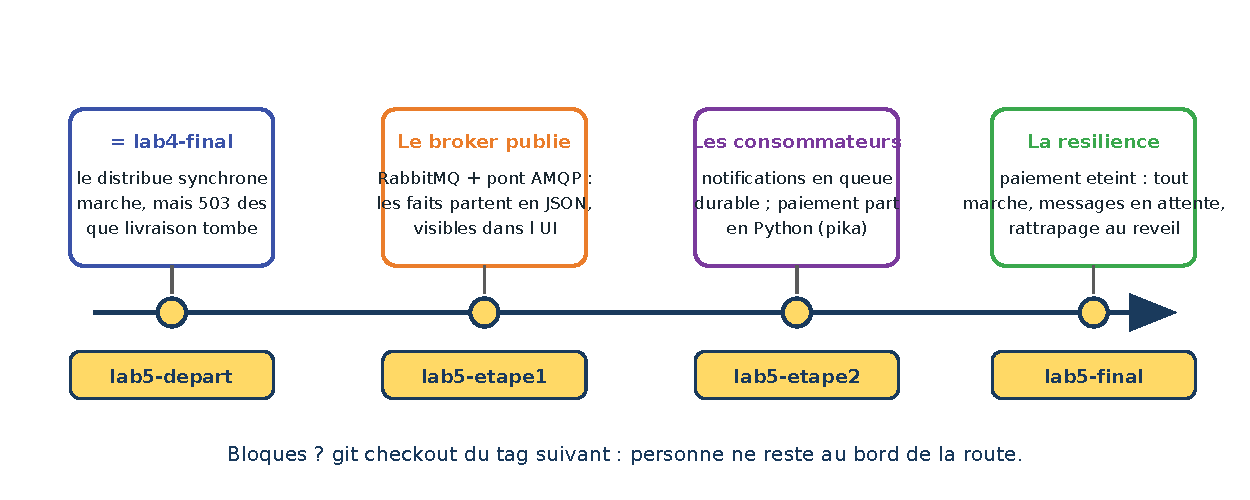
\includegraphics[width=0.80\linewidth]{figP_chemin_lab5}

{\scriptsize Départ : votre \texttt{lab4-final}. Rôles : l'Appariteur pilote \texttt{paiement-service} (pika) ; le Notaire les queues et bindings ; l'Huissier compose + RabbitMQ ; le Rédacteur l'UI de gestion et la preuve du rattrapage ; le Doyen la démo finale et l'\textbf{ADR n\textsuperscript{o}5 : « Synchrone ou asynchrone ? »} — le tableau de décision de \emph{toutes} vos intégrations.}
\end{frame}

\begin{frame}{L'essentiel — et l'arc du semestre}
\begin{ucadret}[À retenir de la séance]
{\footnotesize Un \textbf{broker} transforme les pannes en retards : queue durable + ack = \emph{at-least-once}, dont le prix est l'\textbf{idempotence}. La règle de décision : il faut une réponse $\Rightarrow$ synchrone (et l'on assume le couplage temporel) ; on informe d'un fait $\Rightarrow$ asynchrone (et les consommateurs vivent leur vie).}
\end{ucadret}
\begin{ucadfront}[Le chemin parcouru en cinq séances]
{\footnotesize Un God controller qui souffrait (S1) $\to$ des couches qui séparent la technique (S1) $\to$ un hexagone qui protège le métier (S2) $\to$ des modules aux frontières gardées par un test (S3) $\to$ un premier microservice, extrait avec précaution et payé au prix du synchrone (S4) $\to$ des événements qui voyagent, et des services qui ne meurent plus ensemble (S5). Vous n'avez pas appris \emph{des} architectures : vous avez appris à \textbf{faire évoluer} une architecture — sous tests, par étapes, chaque décision tracée dans un ADR. C'est exactement le métier.}
\end{ucadfront}
\end{frame}

\end{document}
